% -*- TeX-engine: xetex; -*-
% Compile with XeLaTeX

%%%%%%%%%%%%%%%%%%%%%%%
% To do before class
%%%%%%%%%%%%%%%%%%%%%%%

% Send the Logistics/Week0Annoucnement (the night before).
% Send an email reminding students to bring a charged computer (the night before).

%%%%%%%%%%%%%%%%%%%%%%%
% Option 1: Slides: (comment for handouts)   %
%%%%%%%%%%%%%%%%%%%%%%%

\documentclass[slidestop,compress,mathserif,12pt,t,professionalfonts,xcolor=table]{beamer}

% solution stuff
\newcommand{\solnMult}[1]{
\only<1>{#1}
\only<2->{\red{\textbf{#1}}}
}
\newcommand{\soln}[1]{\textit{#1}}

%%%%%%%%%%%%%%%%%%%%%%%%%%%%%%%
% Option 2: Handouts, without solutions (post before class)    %
%%%%%%%%%%%%%%%%%%%%%%%%%%%%%%%

% \documentclass[11pt,containsverbatim,handout,xcolor=xelatex,dvipsnames,table]{beamer}

% % handout layout
% \usepackage{pgfpages}
% \pgfpagesuselayout{4 on 1}[letterpaper,landscape,border shrink=5mm]

% % solution stuff
% \newcommand{\solnMult}[1]{#1}
% \newcommand{\soln}[1]{}

% % % This breaks things for me for some reason.
% % tell pgfpages how to set page sizes in XeLaTeX
% %\renewcommand\pgfsetupphysicalpagesizes{%
% %   \pdfpagewidth\pgfphysicalwidth\pdfpageheight\pgfphysicalheight%
% %}

%%%%%%%%%%%%%%%%%%%%%%%%%%%%%%%%%%%%
% Option 3: Handouts, with solutions (may post after class if need be)    %
%%%%%%%%%%%%%%%%%%%%%%%%%%%%%%%%%%%%

% \documentclass[11pt,containsverbatim,handout,xcolor=xelatex,dvipsnames,table]{beamer}

% % handout layout
% \usepackage{pgfpages}
% \pgfpagesuselayout{4 on 1}[letterpaper,landscape,border shrink=5mm]

% % solution stuff
% \newcommand{\solnMult}[1]{\red{\textbf{#1}}}
% \newcommand{\soln}[1]{\textit{#1}}

% % % This breaks things for me for some reason.
% % % tell pgfpages how to set page sizes in XeLaTeX
% % \renewcommand\pgfsetupphysicalpagesizes{%
% %    \pdfpagewidth\pgfphysicalwidth\pdfpageheight\pgfphysicalheight%
% % }

%%%%%%%%%%%%%%%%%%%%%%%%%%%%%%%
% Option 4: Notes Only
%%%%%%%%%%%%%%%%%%%%%%%%%%%%%%%

% % See http://tex.stackexchange.com/questions/114219/add-notes-to-latex-beamer
% \documentclass[10pt,containsverbatim,xcolor=xelatex,dvipsnames,table,notes=only]{beamer}

% % handout layout
% % \usepackage{pgfpages}
% % \pgfpagesuselayout{1 on 1}[letterpaper, landscape, border shrink=5mm]

% % solution stuff
% \newcommand{\solnMult}[1]{#1}
% \newcommand{\soln}[1]{}

% % % Having a problem with this.
% % tell pgfpages how to set page sizes in XeLaTeX
% % \renewcommand\pgfsetupphysicalpagesizes{%
% %   \pdfpagewidth\pgfphysicalwidth\pdfpageheight\pgfphysicalheight%
% %}

%%%%%%%%%%
% Load style file, defaults  %
%%%%%%%%%%

%%%%%%%%%%%%%%%%
% Themes
%%%%%%%%%%%%%%%%

% See http://deic.uab.es/~iblanes/beamer_gallery/ for mor options

% Style theme
\usetheme{Pittsburgh}

% Color theme
\usecolortheme{seahorse}

% Font theme
%\usepackage[T1]{fontenc}
%\usepackage[scaled=0.92]{helvet}

%\usepackage[no-math]{fontspec}
%\setsansfont{TeX Gyre Heros}
% "TeX Gyre Heros can be used as a replacement for Helvetica"
% In Unix, unzip the following into ~/.fonts
% In Mac, unzip it, double-click the .otf files, and install using "FontBook"
%   http://www.gust.org.pl/projects/e-foundry/tex-gyre/heros/qhv2.004otf.zip

\usepackage{fontspec}

%%%%%%%%%%%%%%%%
% Packages
%%%%%%%%%%%%%%%%

\usepackage{geometry}
\usepackage{graphicx}
\usepackage{amssymb}
\usepackage{epstopdf}
\usepackage{amsmath}  	% this permits text in eqnarray among other benefits
\usepackage{url}		% produces hyperlinks
\usepackage[english]{babel}
\usepackage[latin1]{inputenc}
\usepackage{colortbl}	% allows for color usage in tables
\usepackage{multirow}	% allows for rows that span multiple rows in tables
\usepackage{color}		% this package has a variety of color options
\usepackage{colortbl}
\usepackage{pgf}
\usepackage{calc}
\usepackage{ulem}
\usepackage{multicol}
\usepackage{textcomp}
\usepackage{txfonts}
\usepackage{listings}
\usepackage{tikz}
\usepackage{fancyvrb}

%%%%%%%%%%%%%%%%
% Remove navigation symbols
%%%%%%%%%%%%%%%%

\beamertemplatenavigationsymbolsempty
\hypersetup{pdfpagemode=UseNone} % don't show bookmarks on initial view

%%%%%%%%%%%%%%%%
% User defined colors
%%%%%%%%%%%%%%%%

% Pantone 2015 Spring colors
% http://iwork3.us/2014/09/16/pantone-2015-spring-fashion-report/
% update each semester or year

\xdefinecolor{custom_blue}{rgb}{0, 0.70, 0.79} % scuba blue
\xdefinecolor{custom_darkBlue}{rgb}{0.11, 0.31, 0.54} % classic blue
\xdefinecolor{custom_orange}{rgb}{0.97, 0.57, 0.34} % tangerine
\xdefinecolor{custom_green}{rgb}{0.49, 0.81, 0.71} % lucite green
\xdefinecolor{custom_red}{rgb}{0.58, 0.32, 0.32} % marsala

\xdefinecolor{custom_lightGray}{rgb}{0.78, 0.80, 0.80} % glacier gray
\xdefinecolor{custom_darkGray}{rgb}{0.54, 0.52, 0.53} % titanium

%%%%%%%%%%%%%%%%
% Template colors
%%%%%%%%%%%%%%%%

\setbeamercolor*{palette primary}{fg=white,bg= custom_blue}
\setbeamercolor*{palette secondary}{fg=black,bg= custom_blue!80!black}
\setbeamercolor*{palette tertiary}{fg=white,bg= custom_blue!80!black!80}
\setbeamercolor*{palette quaternary}{fg=white,bg= custom_blue}

\setbeamercolor{structure}{fg= custom_blue}
\setbeamercolor{frametitle}{bg= custom_blue!90}
\setbeamertemplate{blocks}[shadow=false]
\setbeamersize{text margin left=2em,text margin right=2em}

%%%%%%%%%%%%%%%%
% Styling fonts, bullets, etc.
%%%%%%%%%%%%%%%%

% styling of itemize bullets
\setbeamercolor{item}{fg=custom_blue}
\setbeamertemplate{itemize item}{{{\small$\blacktriangleright$}}}
\setbeamercolor{subitem}{fg=custom_blue}
\setbeamertemplate{itemize subitem}{{\textendash}}
\setbeamerfont{itemize/enumerate subbody}{size=\footnotesize}
\setbeamerfont{itemize/enumerate subitem}{size=\footnotesize}

% styling of enumerate bullets
\setbeamertemplate{enumerate item}{\insertenumlabel.}
\setbeamerfont{enumerate item}{family={\fontspec{Helvetica Neue}}}
\setbeamerfont{enumerate subitem}{family={\fontspec{Helvetica Neue}}}
\setbeamerfont{enumerate subsubitem}{family={\fontspec{Helvetica Neue}}}

% make frame titles small to make room in the slide
\setbeamerfont{frametitle}{size=\small} 

% set Helvetica Neue font for frame and section titles
\setbeamerfont{frametitle}{family={\fontspec{Helvetica Neue}}}
\setbeamerfont{sectiontitle}{family={\fontspec{Helvetica Neue}}}
\setbeamerfont{section in toc}{family={\fontspec{Helvetica Neue}}}
\setbeamerfont{subsection in toc}{family={\fontspec{Helvetica Neue}}, size=\small}
\setbeamerfont{footline}{family={\fontspec{Helvetica Neue}}}
\setbeamerfont{subsection in toc}{family={\fontspec{Helvetica Neue}}}
\setbeamerfont{block title}{family={\fontspec{Helvetica Neue}}}

%%%%%%%%%%%%%%%%
% Color text commands
%%%%%%%%%%%%%%%%

%orange
\newcommand{\orange}[1]{\textit{\textcolor{custom_orange}{#1}}}

% green
\newcommand{\green}[1]{\textit{\textcolor{custom_green}{#1}}}

% red
\newcommand{\red}[1]{\textit{\textcolor{custom_red}{#1}}}

% dark gray
\newcommand{\darkgray}[1]{\textit{\textcolor{custom_darkGray}{#1}}}

% light gray
\newcommand{\lightgray}[1]{\textit{\textcolor{custom_lightGray}{#1}}}


%%%%%%%%%%%%%%%%
% Custom commands
%%%%%%%%%%%%%%%%

% cancel
\newcommand{\cancel}[1]{%
    \tikz[baseline=(tocancel.base)]{
        \node[inner sep=0pt,outer sep=0pt] (tocancel) {#1};
        \draw[red, line width=0.5mm] (tocancel.south west) -- (tocancel.north east);
    }%
}

% degree
\newcommand{\degree}{\ensuremath{^\circ}}

% cite
\newcommand{\ct}[1]{
\vfill
{\tiny #1}}

% Note
\newcommand{\Note}[1]{
\rule{2.5cm}{0.25pt} \\ \textit{\footnotesize{\textcolor{custom_red}{Note:} \textcolor{custom_darkGray}{#1}}}}

% Remember
\newcommand{\Remember}[1]{\textit{\scriptsize{\textcolor{custom_red}{Remember:} #1}}}

% links: webURL, webLink
\newcommand{\webURL}[1]{\urlstyle{same}{\textit{\textcolor{custom_blue}{\url{#1}}}}}
\newcommand{\webLink}[2]{\href{#1}{\textcolor{custom_blue}{{#2}}}}

% mail
\newcommand{\mail}[1]{\href{mailto:#1}{\textit{\textcolor{custom_blue}{#1}}}}

% highlighting: hl, hlGr, mathhl
\newcommand{\hl}[1]{\textit{\textcolor{custom_blue}{#1}}}
\newcommand{\hlGr}[1]{\textit{\textcolor{custom_green}{#1}}}
\newcommand{\mathhl}[1]{\textcolor{custom_blue}{\ensuremath{#1}}}

% example
\newcommand{\ex}[1]{\textcolor{blue}{{{\small (#1)}}}}

% two col: two columns
\newenvironment{twocol}[4]{
\begin{columns}[c]
\column{#1\textwidth}
#3
\column{#2\textwidth}
#4
\end{columns}
}

% slot (for probability calculations)
\newenvironment{slot}[2]{
\begin{array}{c} 
\underline{#1} \\ 
#2
\end{array}
}

% pr: left and right parentheses
\newcommand{\pr}[1]{
\left( #1 \right)
}

%%%%%%%%%%%%%%%%
% Custom blocks
%%%%%%%%%%%%%%%%

% activity: less commonly used
\newcommand{\activity}[2]{
\setbeamertemplate{itemize item}{{{\small\textcolor{custom_orange}{$\blacktriangleright$}}}}
\setbeamercolor{block title}{fg=white, bg=custom_orange}
\setbeamerfont{block title}{size=\small}
\setbeamercolor{block body}{fg=black, bg=custom_orange!20!white!80}
\setbeamerfont{block body}{size=\small}
\begin{block}{Activity: #1}
#2
\end{block}
}

% app: application exercise
\newcommand{\app}[2]{
\setbeamercolor{block title}{fg=white,bg=custom_green}
\setbeamercolor{block body}{fg=black,bg=custom_green!20!white!80}
\begin{block}{{\small Application exercise: #1}}
#2
\end{block}
}

% disc: discussion question
\newcommand{\disc}[1]{
\setbeamercolor{block body}{bg=custom_blue!25!white!80, fg=custom_blue!55!black!95}
\begin{block}{\vspace*{-3ex}}
#1
\end{block}
}

% clicker: clicker question
\newcommand{\clicker}[1]{
\setbeamercolor{block title}{bg=custom_blue!80!white!50,fg=custom_blue!30!black!90}
\setbeamercolor{block body}{bg=custom_blue!20!white!80,fg=custom_blue!30!black!90}
\begin{block}{\vspace*{-0.2ex}{\footnotesize Clicker question}\vspace*{-0.2ex}}
#1
\end{block}
}

% formula
\newcommand{\formula}[2]{
\setbeamercolor{block title}{bg=custom_blue!40!white!60,fg=custom_blue!55!black!95}
\begin{block}{{\small#1}}
#2
\end{block}
}

% code
\newcommand{\code}[1]{
\newfontfamily{\monaco}{Monaco}
{\monaco {\footnotesize \textcolor{custom_darkBlue}{#1}}}
}

% output
\renewcommand{\output}[1]{
{\monaco {\footnotesize \textcolor{custom_darkGray}{#1}}}
}

%%%%%%%%%%%%%%%%
% Change margin
%%%%%%%%%%%%%%%%

\newenvironment{changemargin}[2]{%
\begin{list}{}{%
\setlength{\topsep}{0pt}%
\setlength{\leftmargin}{#1}%
\setlength{\rightmargin}{#2}%
\setlength{\listparindent}{\parindent}%
\setlength{\itemindent}{\parindent}%
\setlength{\parsep}{\parskip}%
}%
\item}{\end{list}}

%%%%%%%%%%%%%%%%
% Footnote
%%%%%%%%%%%%%%%%

\long\def\symbolfootnote[#1]#2{\begingroup%
\def\thefootnote{\fnsymbol{footnote}}\footnote[#1]{#2}\endgroup}

%%%%%%%%%%%%%%%%
% Graphics
%%%%%%%%%%%%%%%%

\DeclareGraphicsRule{.tif}{png}{.png}{`convert #1 `dirname #1`/`basename #1 .tif`.png}

%%%%%%%%%%%%%%%%
% Slide number
%%%%%%%%%%%%%%%%

\setbeamertemplate{footline}{%
    \raisebox{5pt}{\makebox[\paperwidth]{\hfill\makebox[20pt]{\color{gray}
          \scriptsize\insertframenumber}}}\hspace*{5pt}}

          
%%%%%%%%%%%%%%%%
% Remove page numbers
%%%%%%%%%%%%%%%%

\newcommand{\removepagenumbers}{% 
  \setbeamertemplate{footline}{}
}

%%%%%%%%%%%%%%%%
% TOC slides
%%%%%%%%%%%%%%%%

% TRY TO CHANGE THE ENUMERATE SYMBOLS HERE FROM CIRCLES TO PLAIN NUMBERS

\AtBeginSection[] 
{ 
  \addtocounter{framenumber}{-1} 
  % 
  {\removepagenumbers 
    \begin{frame}<beamer> 
    \tableofcontents[currentsection] 
  \end{frame} 
  } 
}
% You cannot use numbers when defining variables.  Hence the use of letters, A, B, C, etc.

% Personal Info
\newcommand{\FirstName}{Mine}
\newcommand{\LastName}{\c{C}etinkaya-Rundel}
\newcommand{\OfficeHours}{MTWR 3-4pm.}
\newcommand{\OfficeHoursLocation}{Old Chem 213}

% Electronic Info
\newcommand{\PersonalSite}{http://stat.duke.edu/~mc301}
\newcommand{\CourseSite}{http://bitly.com/sta101sp15}
\newcommand{\Email}{mine@stat.duke.edu}

% TAs
\newcommand{\TAA}{Anthony Weishampel}
\newcommand{\TAB}{Fiamma Li}
\newcommand{\TAC}{Jialiang Mao}
\newcommand{\TAD}{Phillip Lee}

% Exam Dates
\newcommand{\ExamADate}{Wed, Feb 18}
\newcommand{\ExamBDate}{Wed, Mar 25}
\newcommand{\FinalDate}{Sat, May 2 (2-5pm)}

% Due Dates
\newcommand{\ClickerRegistrationDD}{Mon, Jan 26}
\newcommand{\GettingToKnowYouDD}{Friday, Jan 9, 11:59pm}
\newcommand{\ProblemSetADD}{Wed., 1/15}


% ALT ALT
% % You cannot use numbers when defining variables.  Hence the use of letters, A, B, C, etc.

% Personal Info
\renewcommand{\FirstName}{Jesse}
\renewcommand{\LastName}{Windle}
\renewcommand{\OfficeHours}{Tue, Thu 3:00pm-4:30pm}

% Electronic Info
\renewcommand{\PersonalSite}{http://stat.duke.edu/~jbw44/}
\renewcommand{\CourseSite}{http://bitly.com/windle2}
\renewcommand{\Email}{jbw44@stat.duke.edu}

% TAs
\renewcommand{\TAA}{David Clancy}
\renewcommand{\TAB}{Xinyi (Chris) Li}
\renewcommand{\TAC}{Tori Hall}
\renewcommand{\TAD}{Radhika Anand}

% Exam Dates
\renewcommand{\ExamADate}{Thu, Feb 19}
\renewcommand{\ExamBDate}{Thu, Mar 26}
\renewcommand{\FinalDate}{Mon, Apr 27 (9-Noon)}

% Due Dates
\renewcommand{\ClickerRegistrationDD}{Thu, Jan 15}
\renewcommand{\GettingToKnowYouDD}{Friday, Jan 9, 11:59pm}

%%%%%%%%%%%
% Cover slide info    %
%%%%%%%%%%%

\title{Unit 1: Introduction to data}
\subtitle{2. Exploratory data analysis}
\author{Sta 101 - Spring 2015}
\date{January 14, 2015}
\institute{Duke University, Department of Statistical Science}


%%%%%%%%%%%%%%%%%%%%%%%%%
% Begin document and set Helvetica Neue font   %
%%%%%%%%%%%%%%%%%%%%%%%%%

\begin{document}
\fontspec[Ligatures=TeX]{Helvetica Neue Light}

%%%%%%%%%%%%%%%%%%%%%%%%%%%%%%%%%%%

% Title Page

\begin{frame}[plain]

\titlepage
\vfill
{\scriptsize \webLink{\PersonalSite}{Dr. \LastName{}} \hfill Slides posted at  \webLink{\CourseSite}{\CourseSite}}
\addtocounter{framenumber}{-1} 

\end{frame}

%%%%%%%%%%%%%%%%%%%%%%%%%%%%%%%%%%%

\section{Housekeeping}

%%%%%%%%%%%%%%%%%%%%%%%%%%%%%%%%%%%

\begin{frame}
\frametitle{Announcements}

\begin{itemize}

\item Sit in teams in class and lab going forward -- are you missing a team member?

\item If you haven't yet done so, take the class survey

\item Lab 1 due by your lab session next Monday -- one submission per team sufficient
\begin{itemize}
\item Questions about labs?
\end{itemize}

\item TA office hours:
\begin{itemize}

\item SEC open 4pm - 9pm Sunday - Thursday

\item Sta 101 TA hours:
\vspace{-0.25cm}
\begin{multicols}{2}
\begin{itemize}
\item \hl{Christine - Sun, 4-6pm}
\item David - Mon, 4-6pm
\item \hl{Anthony - Mon, 7-9pm}
\item Chris (Xinyi) - Tues, 5-7pm
\item Radhika - Tues, 7-9pm
\item \hl{Mao - Wed, 5-7pm}
\item Tori - Wed, 7-9pm
\item \hl{Fiamma - Thur, 6-7pm}
\item \hl{Phillip - TBA}
\end{itemize}
\end{multicols}
\vspace{-0.25cm}
\end{itemize}

\item No class and no OH on Monday, review randomization test video before Wednesday's class

\item PS 2 due Wednesday

\end{itemize}

\end{frame}

%%%%%%%%%%%%%%%%%%%%%%%%%%%%%%%%%%%

\begin{frame}
\frametitle{From last time - App Ex 1.1: Haters gonna hate}

\begin{enumerate}

\item Cases: 200 men and women
\item Response: Attitude towards the microwave oven
\item Explanatory: Whether the participant is a hater or not
\item Random sampling / assignment: Via Amazon's MTurk - self selected sample, no random assignment.
\item Type: Observational, doesn't use random assignment. 
\item Causality: No
\item Generalizability: Only if we could assume sample from Amazon's MTurk's sample is representative

\end{enumerate}

\end{frame}

%%%%%%%%%%%%%%%%%%%%%%%%%%%%%%%%%%%


\section{Main ideas}

%%%%%%%%%%%%%%%%%%%%%%%%%%%%%%%%%%%

\subsection{Always start your exploration with a visualization}
\label{mi1}

%%%%%%%%%%%%%%%%%%%%%%%%%%%%%%%%%%%

\begin{frame}[fragile]
\frametitle{From your survey...}

\disc{Do you see anything out of the ordinary?}

\begin{center}
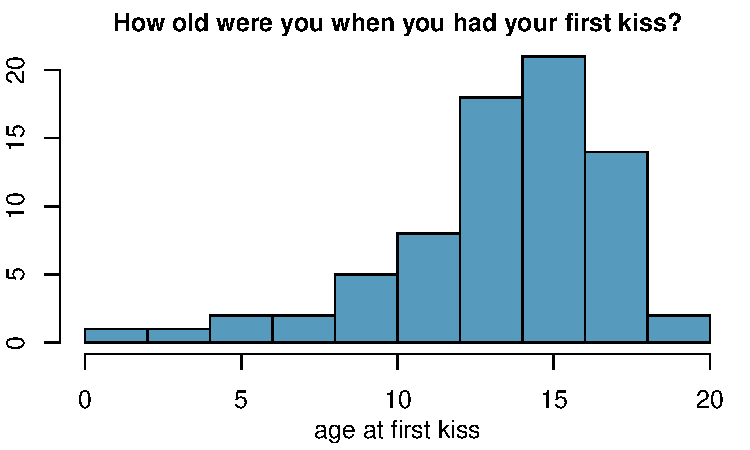
\includegraphics[width=0.8\textwidth]{figures/survey/hist_first_kiss} 
\end{center}

\pause

\soln{Some people reported very low ages, which might suggest the survey question wasn't clear: romantic kiss or any kiss?}

\end{frame}

%%%%%%%%%%%%%%%%%%%%%%%%%%%%%%%%%%%

\begin{frame}[fragile]
\frametitle{From your survey...}

\disc{How are people reporting lower vs. higher values of FB visits?}

\begin{center}
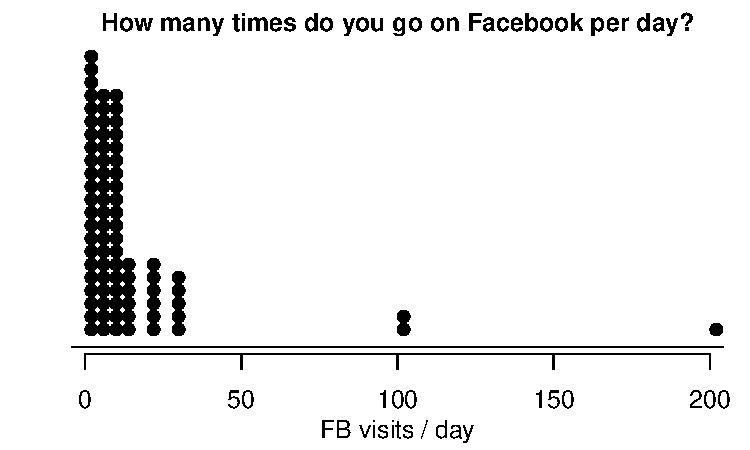
\includegraphics[width=0.8\textwidth]{figures/survey/dot_fb_visits_per_day} 
\end{center}

\pause

\soln{Finer scale for lower numbers.}

\end{frame}

%%%%%%%%%%%%%%%%%%%%%%%%%%%%%%%%%%%

\begin{frame}
\frametitle{}

\disc{Describe the spatial distribution of preferred sweetened carbonated beverage drink.}

\begin{center}
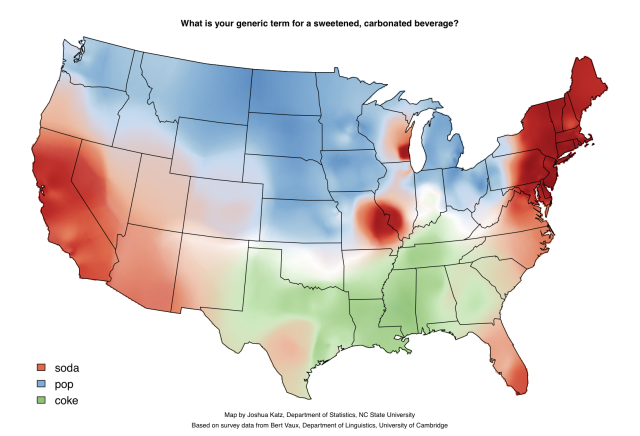
\includegraphics[width=0.9\textwidth]{figures/spatial/soda}
\end{center}

\ct{\webURL{http://spark.rstudio.com/jkatz/SurveyMaps}}

\end{frame}

%%%%%%%%%%%%%%%%%%%%%%%%%%%%%%%%%%%

\begin{frame}
\frametitle{}

\disc{What is missing in this visualization?}

\begin{center}
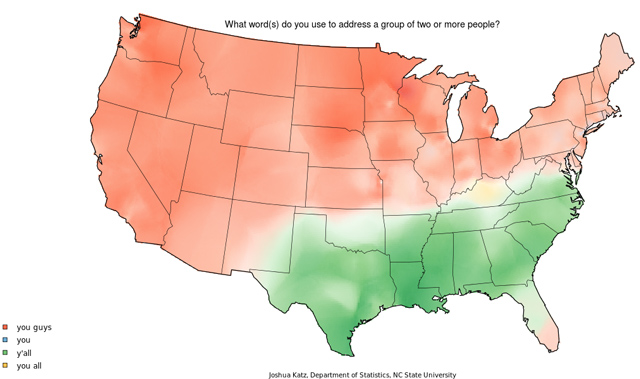
\includegraphics[width=0.9\textwidth]{figures/spatial/yalls}
\end{center}

\ct{\webURL{http://spark.rstudio.com/jkatz/SurveyMaps}}

\end{frame}

%%%%%%%%%%%%%%%%%%%%%%%%%%%%%%%%%%

\subsection{When describing numerical distributions discuss shape, center, spread, and unusual observations}
\label{mi2}

%%%%%%%%%%%%%%%%%%%%%%%%%%%%%%%%%%%

\begin{frame}
\frametitle{Describing distributions of numerical variables}

\begin{itemize}

\item \hl{Shape}: skewness, modality

\item \hl{Center}: an estimate of a \hl{typical} observation in the distribution (mean, median, mode, etc.) 
\begin{itemize}
\item Notation: $\mu$: population mean, $\bar{x}$: sample mean
\end{itemize}

\item \hl{Spread}: measure of variability in the distribution (standard deviation, IQR, range, etc.)

\item \hl{Unusual observations}: observations that stand out from the rest of the data that may be suspected outliers

\end{itemize}

\end{frame}

%%%%%%%%%%%%%%%%%%%%%%%%%%%%%%%%%%

\begin{frame}
\frametitle{}

\clicker{Which of these is most likely to have a roughly symmetric distribution?}

\begin{enumerate}[(a)]
\item salaries of a random sample of people from North Carolina
\item \solnMult{weights of adult females}
\item scores on an well-designed exam
\item last digits of phone numbers
\end{enumerate}

\end{frame}

%%%%%%%%%%%%%%%%%%%%%%%%%%%%%%%%%%%

\begin{frame}
\frametitle{Mean vs. median}

\clicker{How do the mean and median of the following two datasets compare? \\
$\:$\\
Dataset 1: 30, 50, 70, 90 \\
Dataset 2: 30, 50, 70, 1000
}

\begin{enumerate}[(a)]
\item $\bar{x}_1 = \bar{x}_2$, $median_1 = median_2$
\item \solnMult{$\bar{x}_1 < \bar{x}_2$, $median_1 = median_2$}
\item $\bar{x}_1 < \bar{x}_2$, $median_1 < median_2$
\item $\bar{x}_1 > \bar{x}_2$, $median_1 < median_2$
\item $\bar{x}_1 > \bar{x}_2$, $median_1 = median_2$
\end{enumerate}

\end{frame}

%%%%%%%%%%%%%%%%%%%%%%%%%%%%%%%%%%%

\begin{frame}
\frametitle{Standard deviation and variance}

\begin{itemize}

\item Most commonly used measure of variability is the \hl{standard deviation}, which roughly measures the average deviation from the mean
\begin{itemize}
\item Notation: $\sigma$: population standard deviation, $s$: sample standard deviation
\end{itemize}

\item Calculating the standard deviation, for a population (rarely, if ever) and for a sample:

\[ \darkgray{$\sigma = \sqrt{\frac{\sum_{i = 1}^N (x_i - \mu)^2}{n}}$} \qquad s = \sqrt{\frac{\sum_{i = 1}^n (x_i - \bar{x})^2}{n - 1}} \]

\item Square of the standard deviation is called the \hl{variance}.

\end{itemize}

\end{frame}

%%%%%%%%%%%%%%%%%%%%%%%%%%%%%%%%%%%

\begin{frame}
\frametitle{More on SD}

\disc{Why divide by $n - 1$ instead of $n$ when calculating the sample standard deviation?}

\pause

Lose a ``degree of freedom" for using an estimate (the sample mean, $\bar{x}$), in estimating the sample variance/standard deviation.

\pause

$\:$ \\

\disc{Why do we use the squared deviation in the calculation of variance?}

\pause

\begin{itemize}
\item To get rid of negatives so that observations equally distant from the mean are weighed equally.
\item To weigh larger deviations more heavily.
\end{itemize}

\end{frame}

%%%%%%%%%%%%%%%%%%%%%%%%%%%%%%%%%%%

\begin{frame}
\frametitle{Range and IQR}

\clicker{True / False: The range is always larger than the IQR for a given dataset.}

\begin{enumerate}[(a)]
\item \solnMult{Yes}
\item No
\end{enumerate}

\soln{\pause Range = max - min, IQR = Q3 - Q1}

$\:$ \\
\pause

\disc{Is the range or the IQR more robust to outliers?}

\soln{\pause{IQR}}

\end{frame}

%%%%%%%%%%%%%%%%%%%%%%%%%%%%%%%%%%%

\subsection{Robust statistics are not easily affected by outliers and extreme skew}
\label{mi3}

%%%%%%%%%%%%%%%%%%%%%%%%%%%%%%%%%%%

\begin{frame}
\frametitle{Robust statistics}

\begin{itemize}

\item Mean and standard deviation are easily affected by extreme observations since the value of each data point contributes to their calculation.

\item Median and IQR are more robust.

\item Therefore we choose median\&IQR (over mean\&SD) when describing skewed distributions.

\end{itemize}

\end{frame}

%%%%%%%%%%%%%%%%%%%%%%%%%%%%%%%%%%%

\begin{frame}
\frametitle{}

\vfill

\app{1.2 Distributions of numerical variables}{$\:$\\ See the course website for instructions. \\$\:$}

\vfill

\end{frame}

%%%%%%%%%%%%%%%%%%%%%%%%%%%%%%%%%%%

\subsection{Use box plots to display quartiles, median, and outliers}
\label{mi4}

%%%%%%%%%%%%%%%%%%%%%%%%%%%%%%%%%%%

\begin{frame}
\frametitle{Box plot}

A \hl{box plot} visualizes the median, the quartiles, and suspected outliers. An \hl{outlier} is defined as an observation more than 1.5$\times$IQR away from the quartiles.

\begin{center}
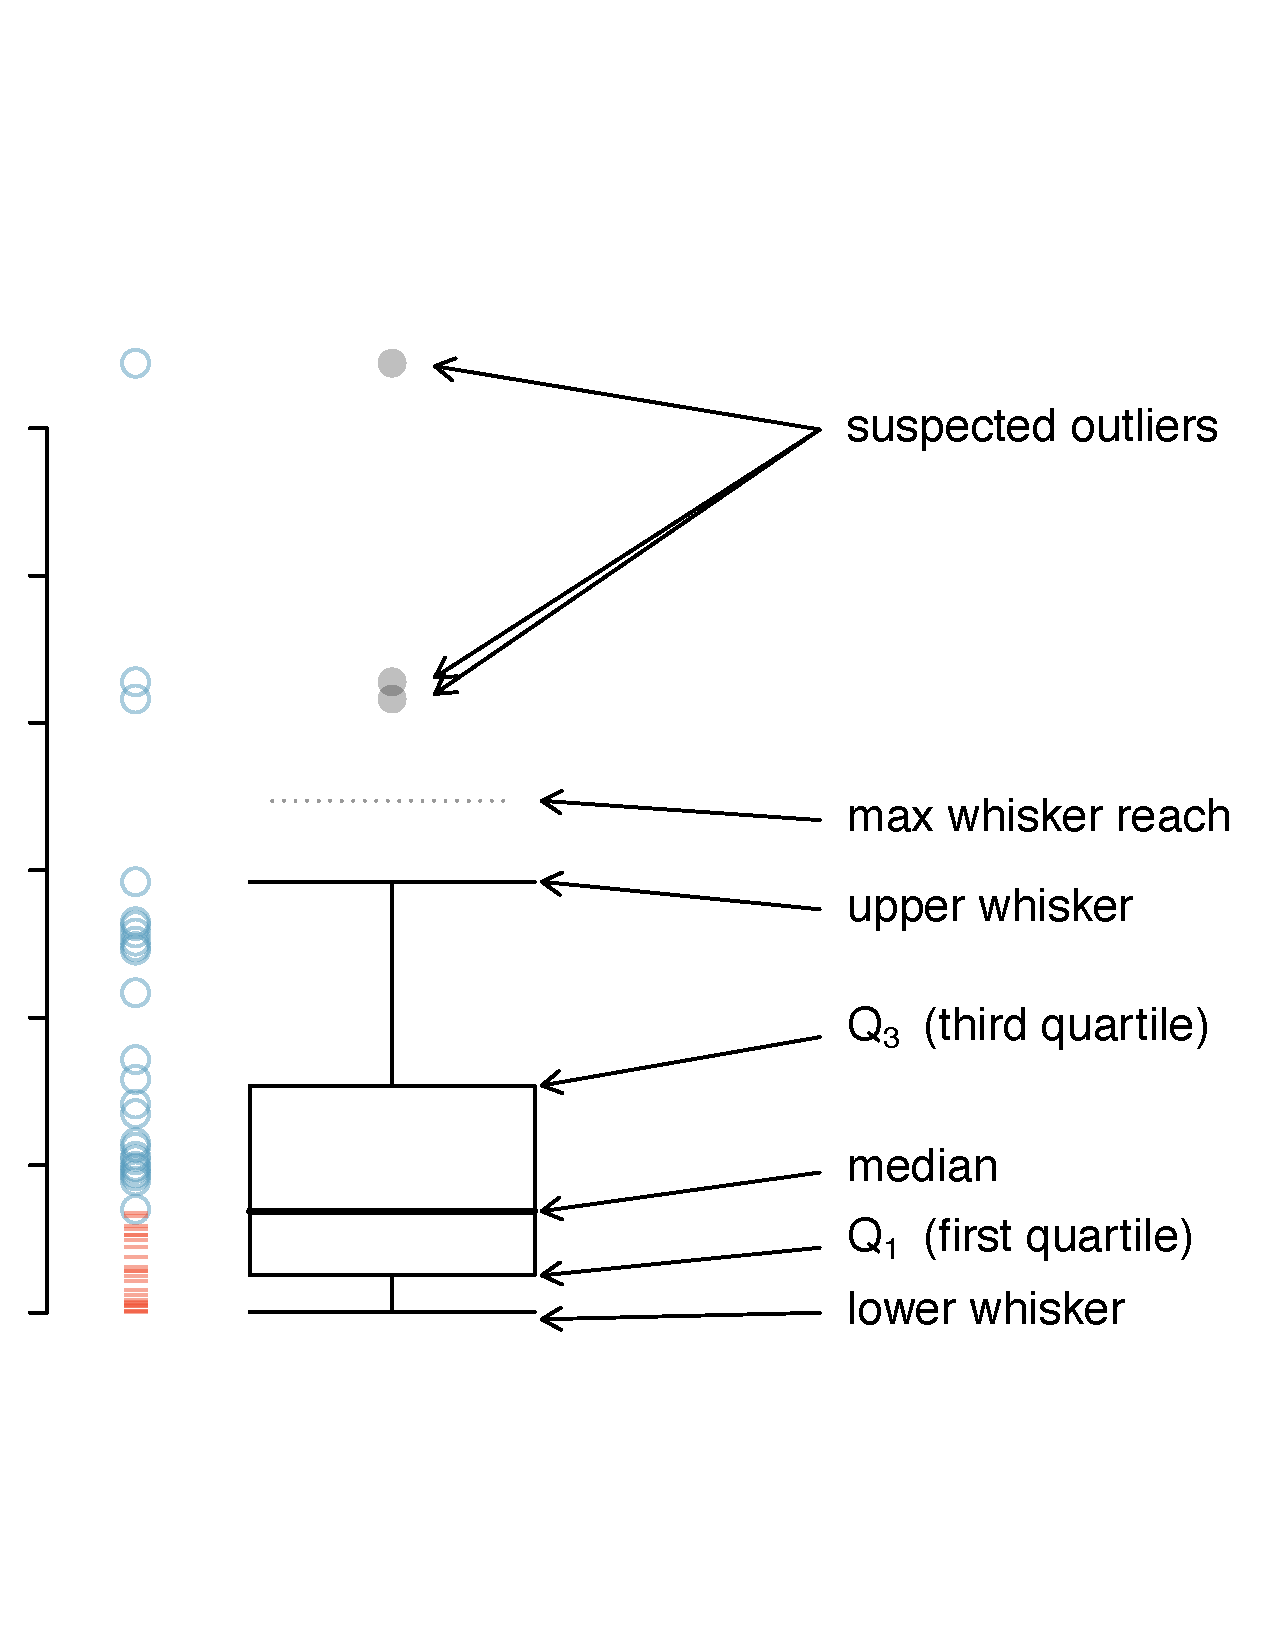
\includegraphics[width=0.6\textwidth]{figures/boxPlotLayoutNumVar}
\end{center}

\end{frame}

%%%%%%%%%%%%%%%%%%%%%%%%%%%%%%%%%%%

\begin{frame}[fragile]
\frametitle{}

\vfill

\app{1.3 Boxplots}{$\:$\\ See the course website for instructions. \\$\:$}

\vfill

\end{frame}

%%%%%%%%%%%%%%%%%%%%%%%%%%%%%%%%%%%

\subsection{Use mosaic plots for visualizing relationship between two categorical variables}
\label{mi5}

%%%%%%%%%%%%%%%%%%%%%%%%%%%%%%%%%%%%

\begin{frame}
\frametitle{}

\disc{What do the widths of the bars represent? What about the heights of the boxes? Is there a relationship between class year and relationship status? What other tools could we use to summarize these data?}

\begin{center}
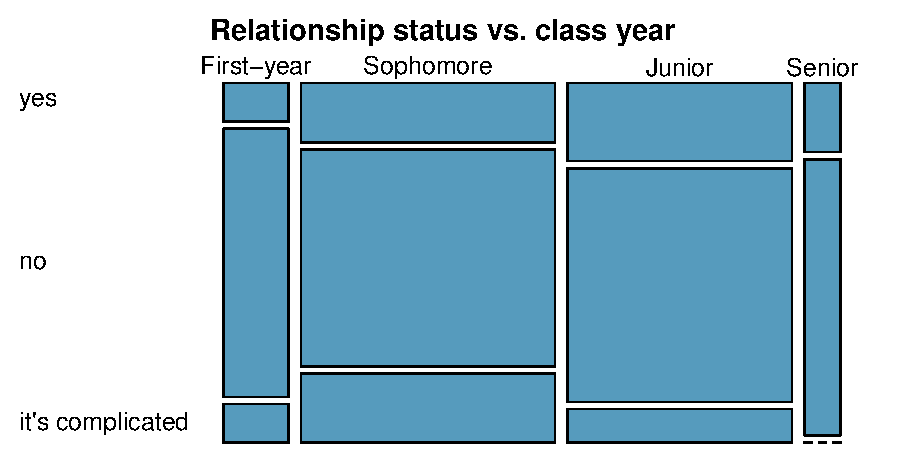
\includegraphics[width=0.9\textwidth]{figures/survey/mosaic_relstatus_class.pdf}
\end{center}

\end{frame}

%%%%%%%%%%%%%%%%%%%%%%%%%%%%%%%%%%%%

\subsection{Be aware of Simpson's paradox}
\label{mi6}

%%%%%%%%%%%%%%%%%%%%%%%%%%%%%%%%%%%%

\begin{frame}
\frametitle{Race and death-penalty sentences in Florida murder cases}

A 1991 study by Radelet and Pierce on race and death-penalty (DP) sentences gives the following table:

\begin{center}
\begin{tabular}{l c c c c}
\hline
Defendant's race 	& DP 	& No DP 	& Total 	& \% DP \\
\hline
Caucasian		& 53		& 430	& 483	& \only<2-|handout:0>{\red{11\%}} \\
African American	& 15		& 176	& 191	& \only<3-|handout:0>{\orange{7.9\%}}  \\ 
\hline
Total				& 68		& 606	& 674 
\end{tabular}
\end{center}

\only<4->{
\disc{Who is more likely to get the death penalty?}
}

\vfill

\ct{Adapted from Subsection 2.3.2 of A. Agresti (2002), Categorical Data Analysis, 2nd ed., and \webURL{http://math.stackexchange.com/questions/83756/examples-of-simpsons-paradox}.}

\end{frame}

%%%%%%%%%%%%%%%%%%%%%%%%%%%%%%%%%%%%

\begin{frame}
\frametitle{Another look}

Same data, taking into consideration victim's race:

{\small
\begin{center}
\begin{tabular}{l l c c c c}
\hline
Victim's race		& Defendant's race 	& DP 	& No DP 	& Total 	& \% DP \\
\hline
Caucasian		& Caucasian		& 53		& 414	& 467	& \only<2-|handout:0>{\orange{11.3\%}} \\
Caucasian		& African American	& 11		& 37		& 48		& \only<3-|handout:0>{\red{22.9\%}}  \\ 
African American	& Caucasian		& 0		& 16		& 16		& \only<4-|handout:0>{\orange{0\%}}  \\ 
African American	& African American	& 4		& 139	& 143	& \only<5-|handout:0>{\red{2.8\%}}  \\ 
\hline
Total				&				& 68		& 606	& 674 
\end{tabular}
\end{center}
}

\only<6->{
\disc{Who is more likely to get the death penalty?}
}

\end{frame}

%%%%%%%%%%%%%%%%%%%%%%%%%%%%%%%%%%%%

\begin{frame}
\frametitle{Contradiction?}

\begin{itemize}

\item People of one race are more likely to murder others of the same race, murdering a Caucasian is more likely to result in the death penalty, and there are more Caucasian defendants than African American defendants in the sample.

\pause

\item Controlling for the victim's race reveals more insights into the data, and changes the direction of the relationship between race and death penalty.

\pause

\item This phenomenon is called \hl{Simpson's Paradox}: An association, or a comparison, that holds when we compare two groups can disappear or even be reversed when the original groups are broken down into smaller groups according to some other feature (a confounding/lurking variable).

\end{itemize}


\end{frame}

%%%%%%%%%%%%%%%%%%%%%%%%%%%%%%%%%%%%

\subsection{Use side-by-side box plots to visualize relationships between numerical and categorical variables}
\label{mi7}

%%%%%%%%%%%%%%%%%%%%%%%%%%%%%%%%%%%%

\begin{frame}[fragile]
\frametitle{Side-by-side box plot}

\disc{How do drinking habits of vegetarian vs. non-vegetarian students compare?}

\begin{center}
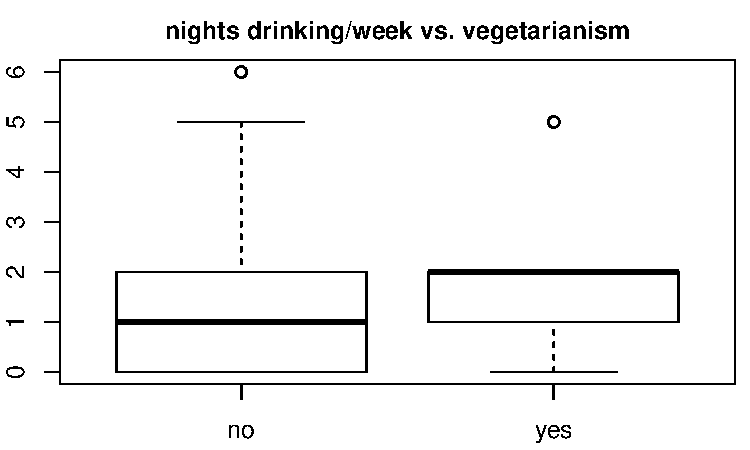
\includegraphics[width=0.9\textwidth]{figures/survey/box_drinks_veg}
\end{center}

\end{frame}

%%%%%%%%%%%%%%%%%%%%%%%%%%%%%%%%%%%%

\section{Summary}

%%%%%%%%%%%%%%%%%%%%%%%%%%%%%%%%%%%%

\begin{frame}
\frametitle{Summary of main ideas}

\vfill

\begin{enumerate}

\item \nameref{mi1}

\item \nameref{mi2}

\item \nameref{mi3}

\item \nameref{mi4}

\item \nameref{mi5}

\item \nameref{mi6}

\item \nameref{mi7}

\end{enumerate}

\vfill

\end{frame}

%%%%%%%%%%%%%%%%%%%%%%%%%%%%%%%%%%%

\end{document}